\newpage
\chapter{Осциллограммы и спектры}

\section{Амплитудная модуляция}

\begin{figure}[H]
    \centering
    % Замените на имя вашего файла с графиком
    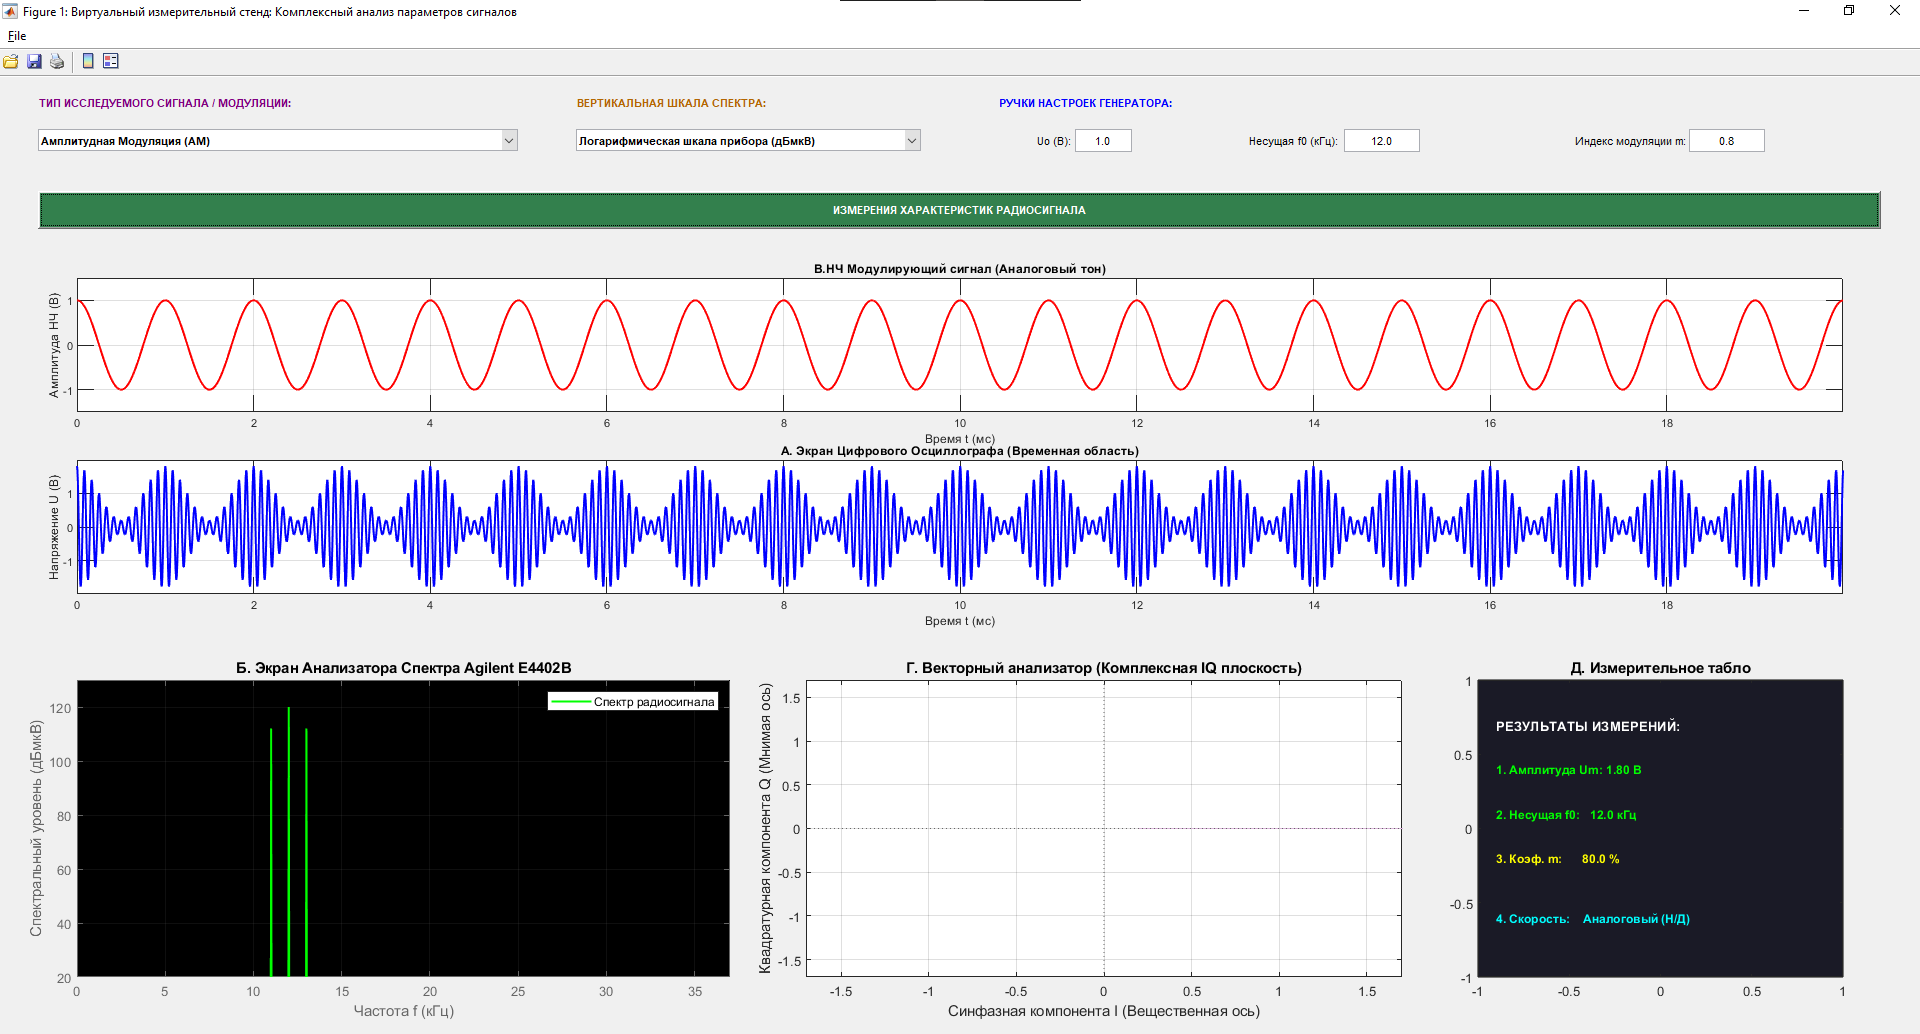
\includegraphics[width=1.0\textwidth]{images/AM_0.8}
    \caption{Осциллограмма, спектр и векторная IQ-диаграмма АМ-сигнала при $m = 0.8$}
    \label{fig:AM_0.8}
\end{figure}

\begin{figure}[H]
    \centering
    % Замените на имя вашего файла с графиком
    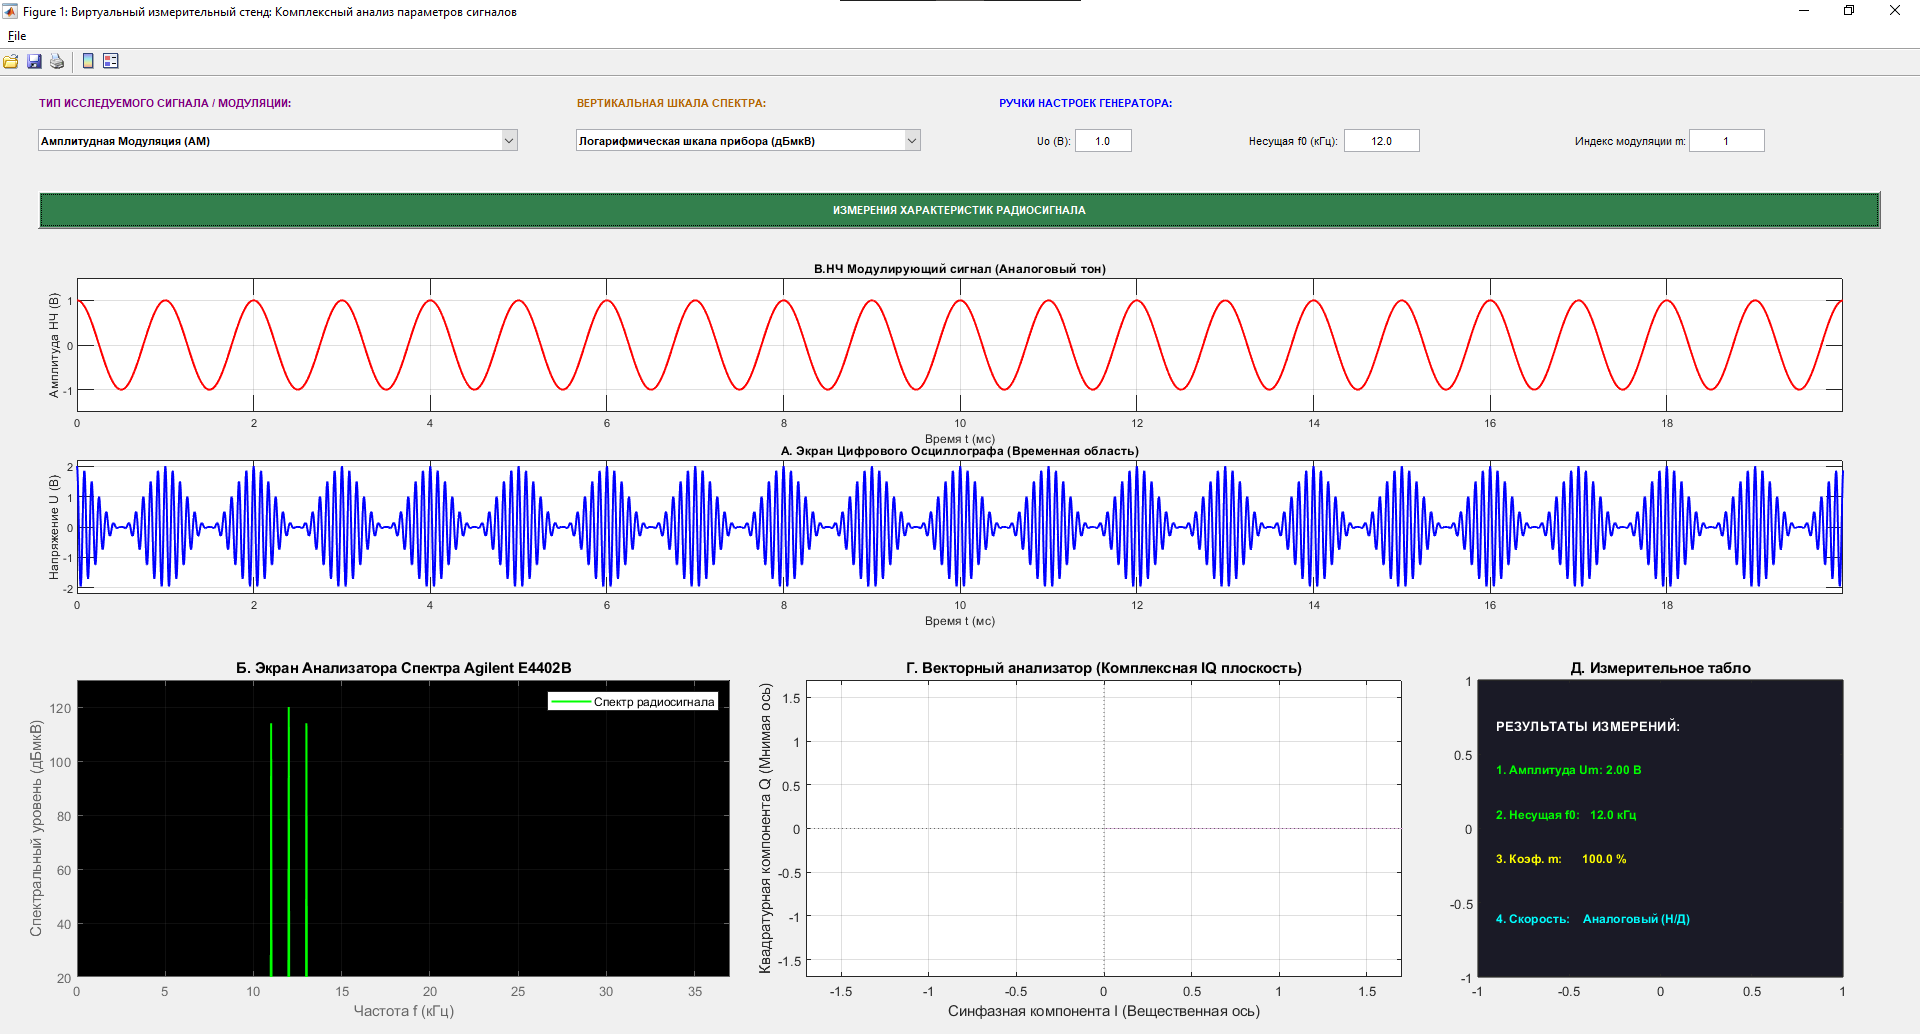
\includegraphics[width=1.0\textwidth]{images/AM_1.0}
    \caption{Временная и частотная характеристики АМ-сигнала при предельной модуляции $m = 1.0$}
    \label{fig:AM_1.0}
\end{figure}

\section{Частотная модуляция}

\begin{figure}[H]
    \centering
    % Замените на имя вашего файла с графиком
    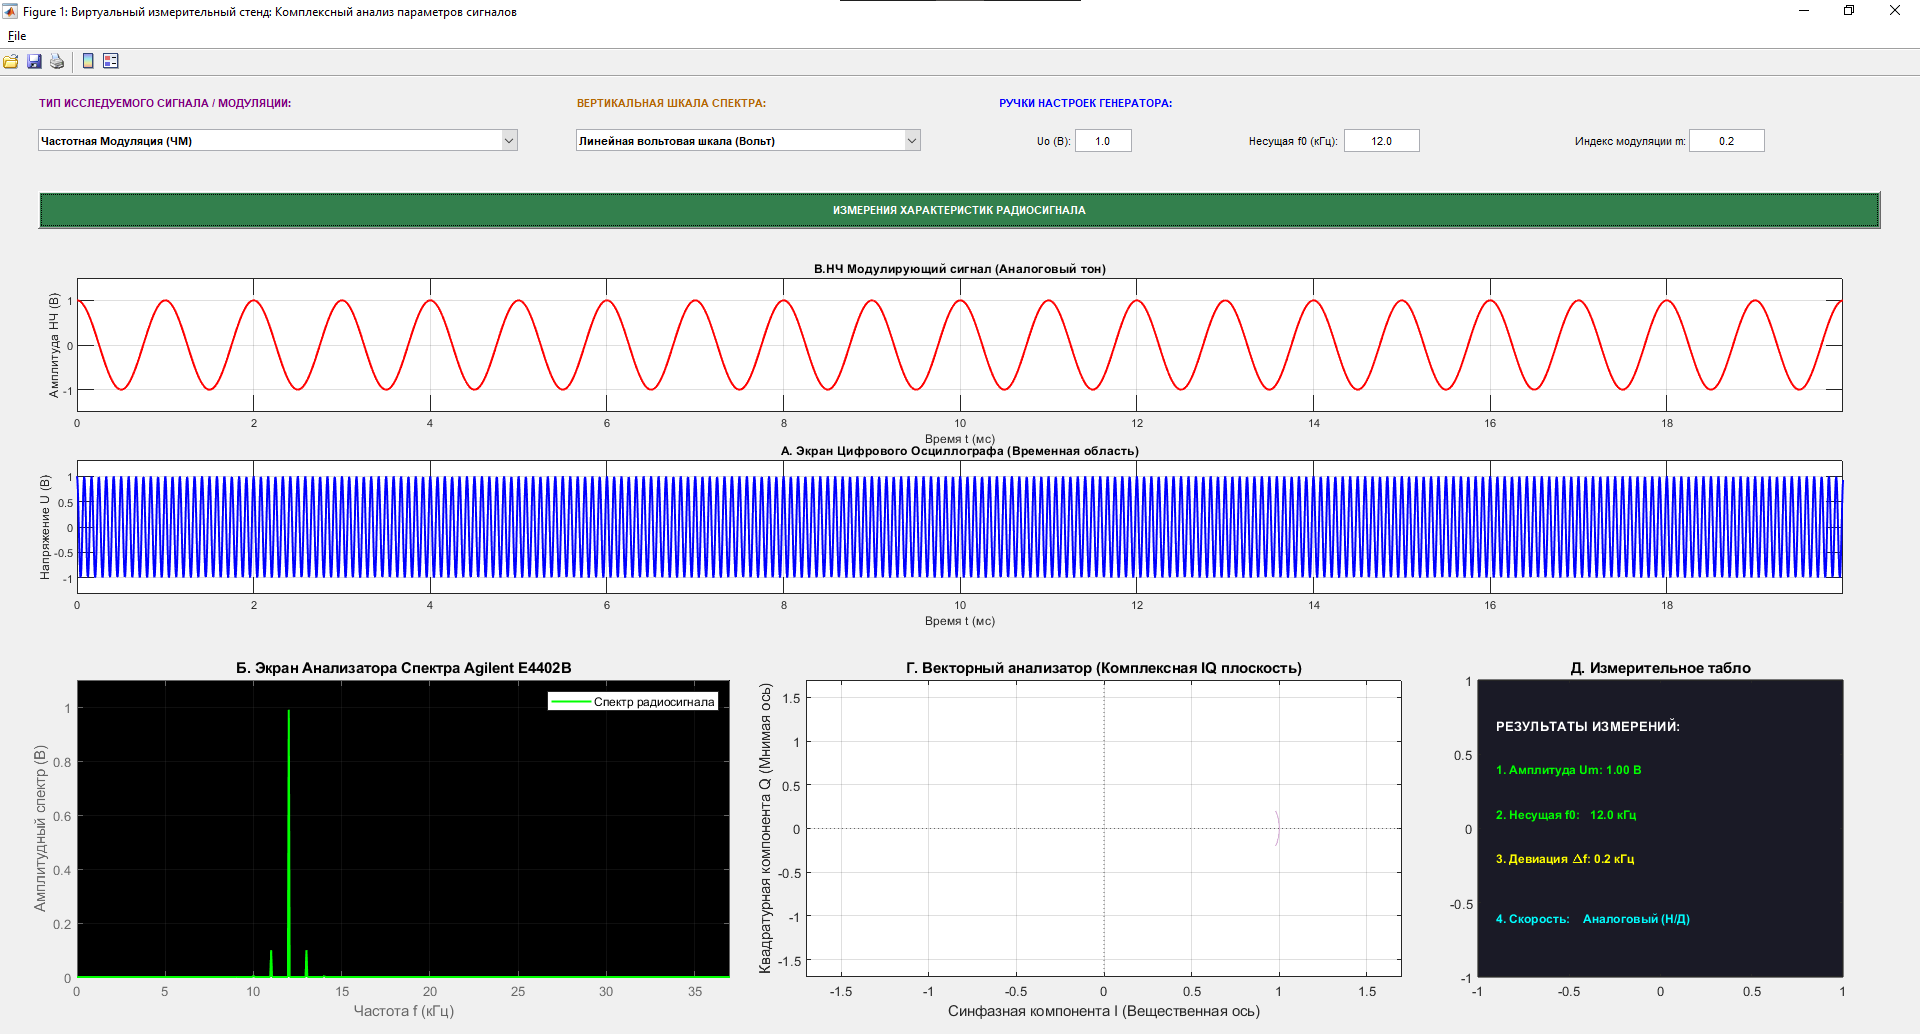
\includegraphics[width=1.0\textwidth]{images/ChM_0.2}
    \caption{Осциллограмма, спектр и фазовый портрет ЧМ-сигнала при $m = 0.2$}
    \label{fig:ChM_0.2}
\end{figure}

\begin{figure}[H]
    \centering
    % Замените на имя вашего файла с графиком
    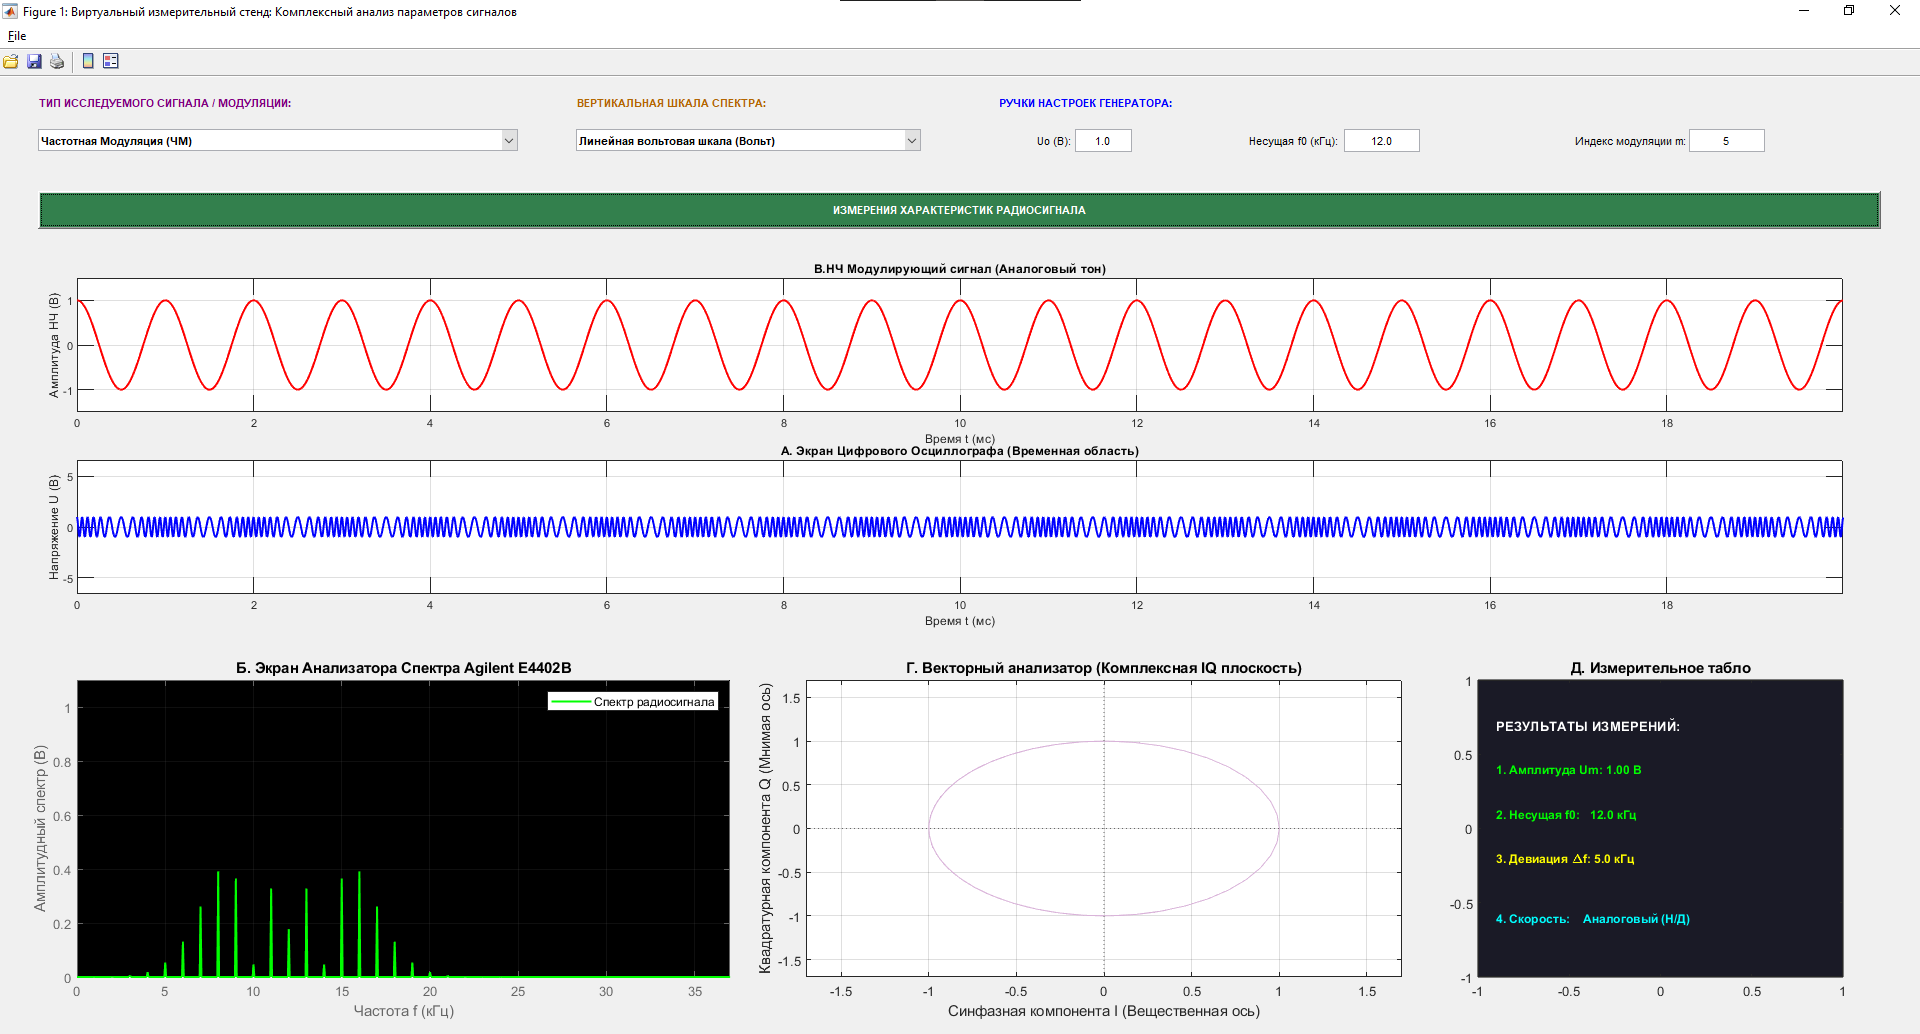
\includegraphics[width=1.0\textwidth]{images/ChM_5.0}
    \caption{Временная реализация, широкий многополосный спектр и кольцевой фазовый портрет ЧМ-сигнала при $m = 5.0$}
    \label{fig:ChM_5.0}
\end{figure}

\section{Фазовая модуляция}

\begin{figure}[H]
    \centering
    % Замените на имя вашего файла с графиком
    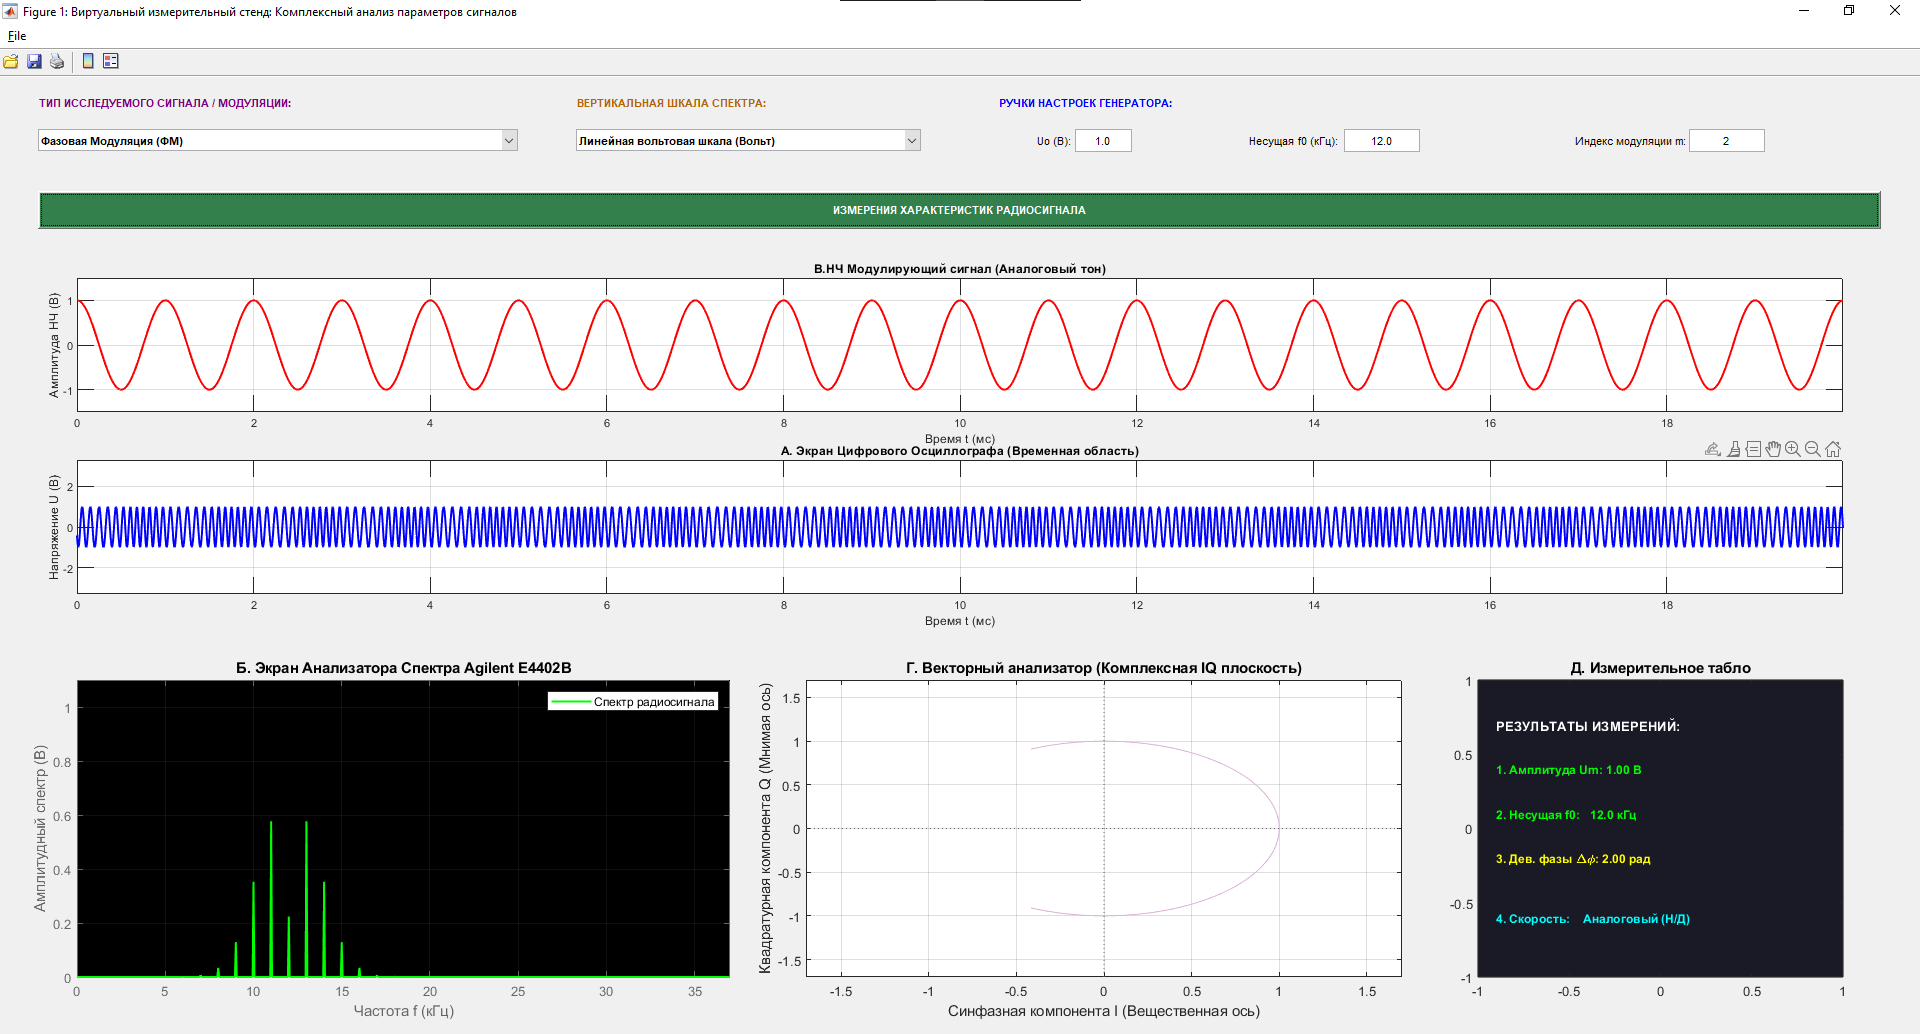
\includegraphics[width=1.0\textwidth]{images/PM_2.0}
    \caption{Осциллограмма, спектр и фазовый портрет ФМ-сигнала при $m = 2.0$}
    \label{fig:PM_2.0}
\end{figure}

\begin{figure}[H]
    \centering
    % Замените на имя вашего файла с графиком
    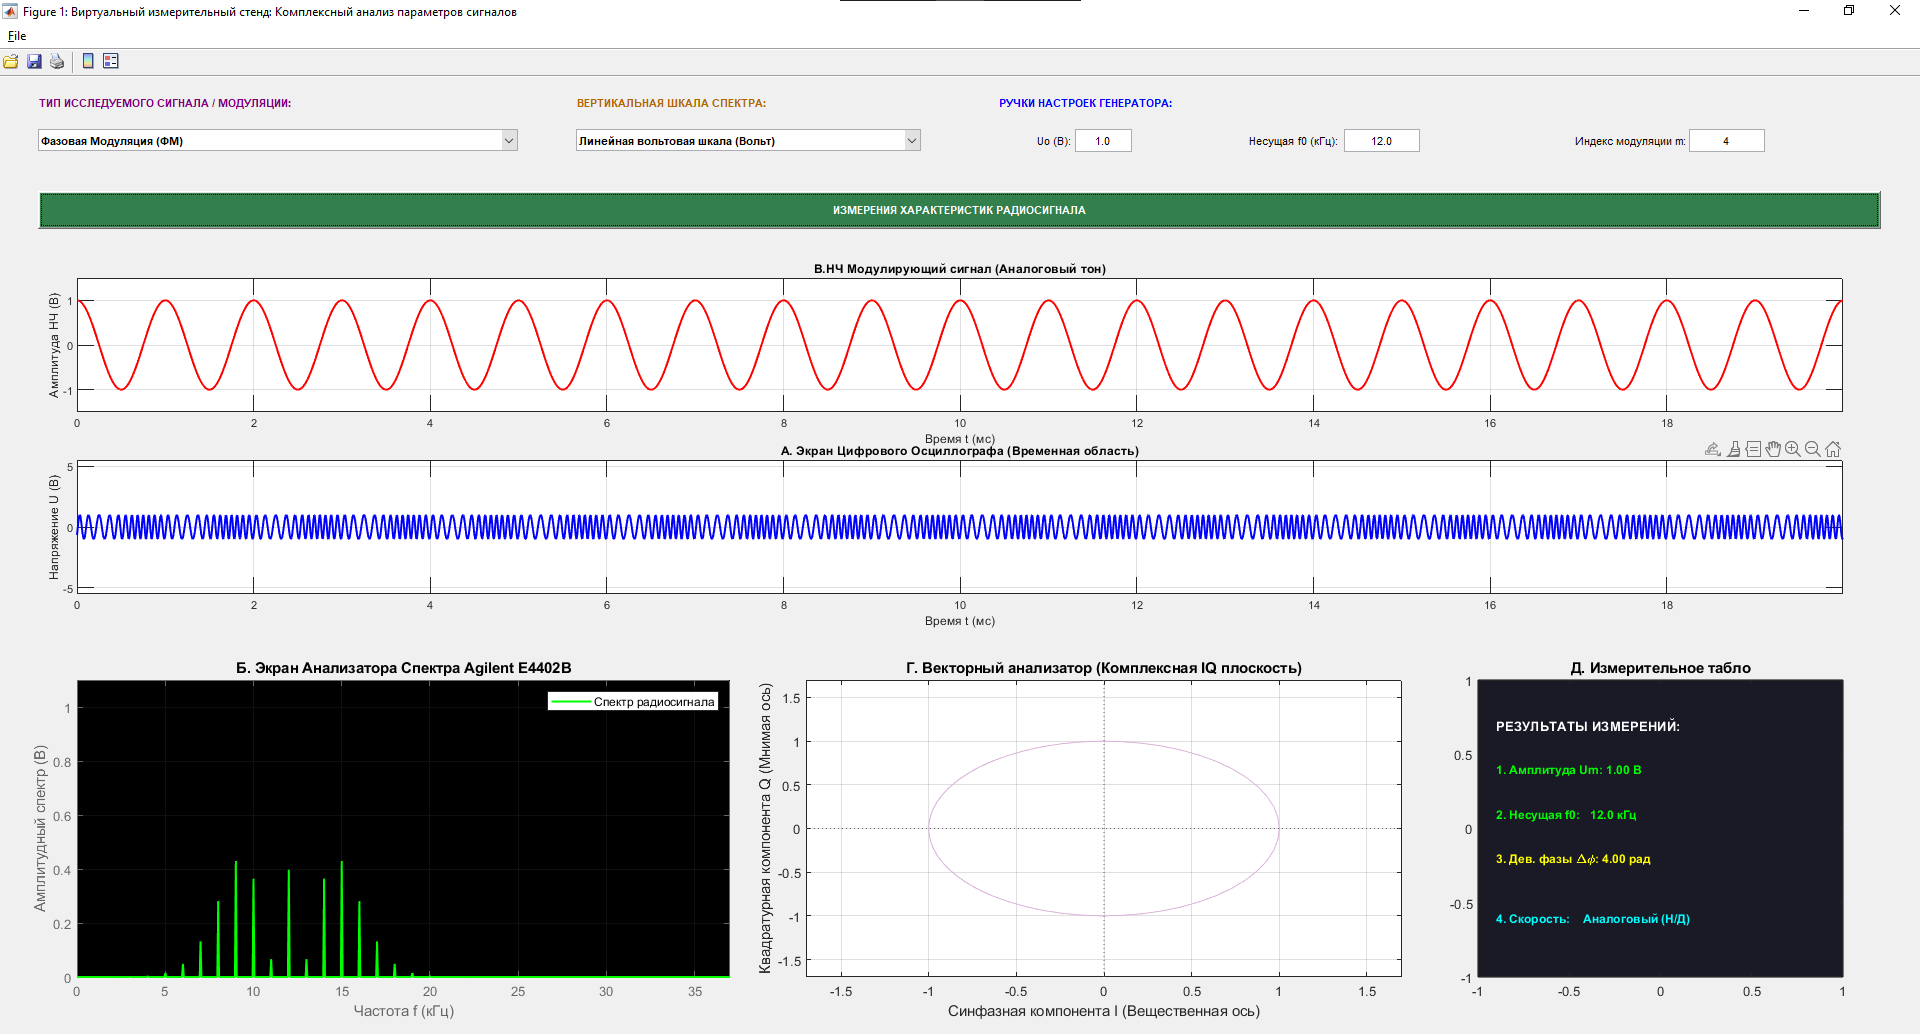
\includegraphics[width=1.0\textwidth]{images/PM_4.0}
    \caption{Осциллограмма, спектр и замкнутый кольцевой фазовый портрет ФМ-сигнала при $m = 4.0$}
    \label{fig:PM_4.0}
\end{figure}

\section{Двухпозиционная фазовая манипуляция}

\begin{figure}[H]
    \centering
    % Замените на имя вашего файла с графиком
    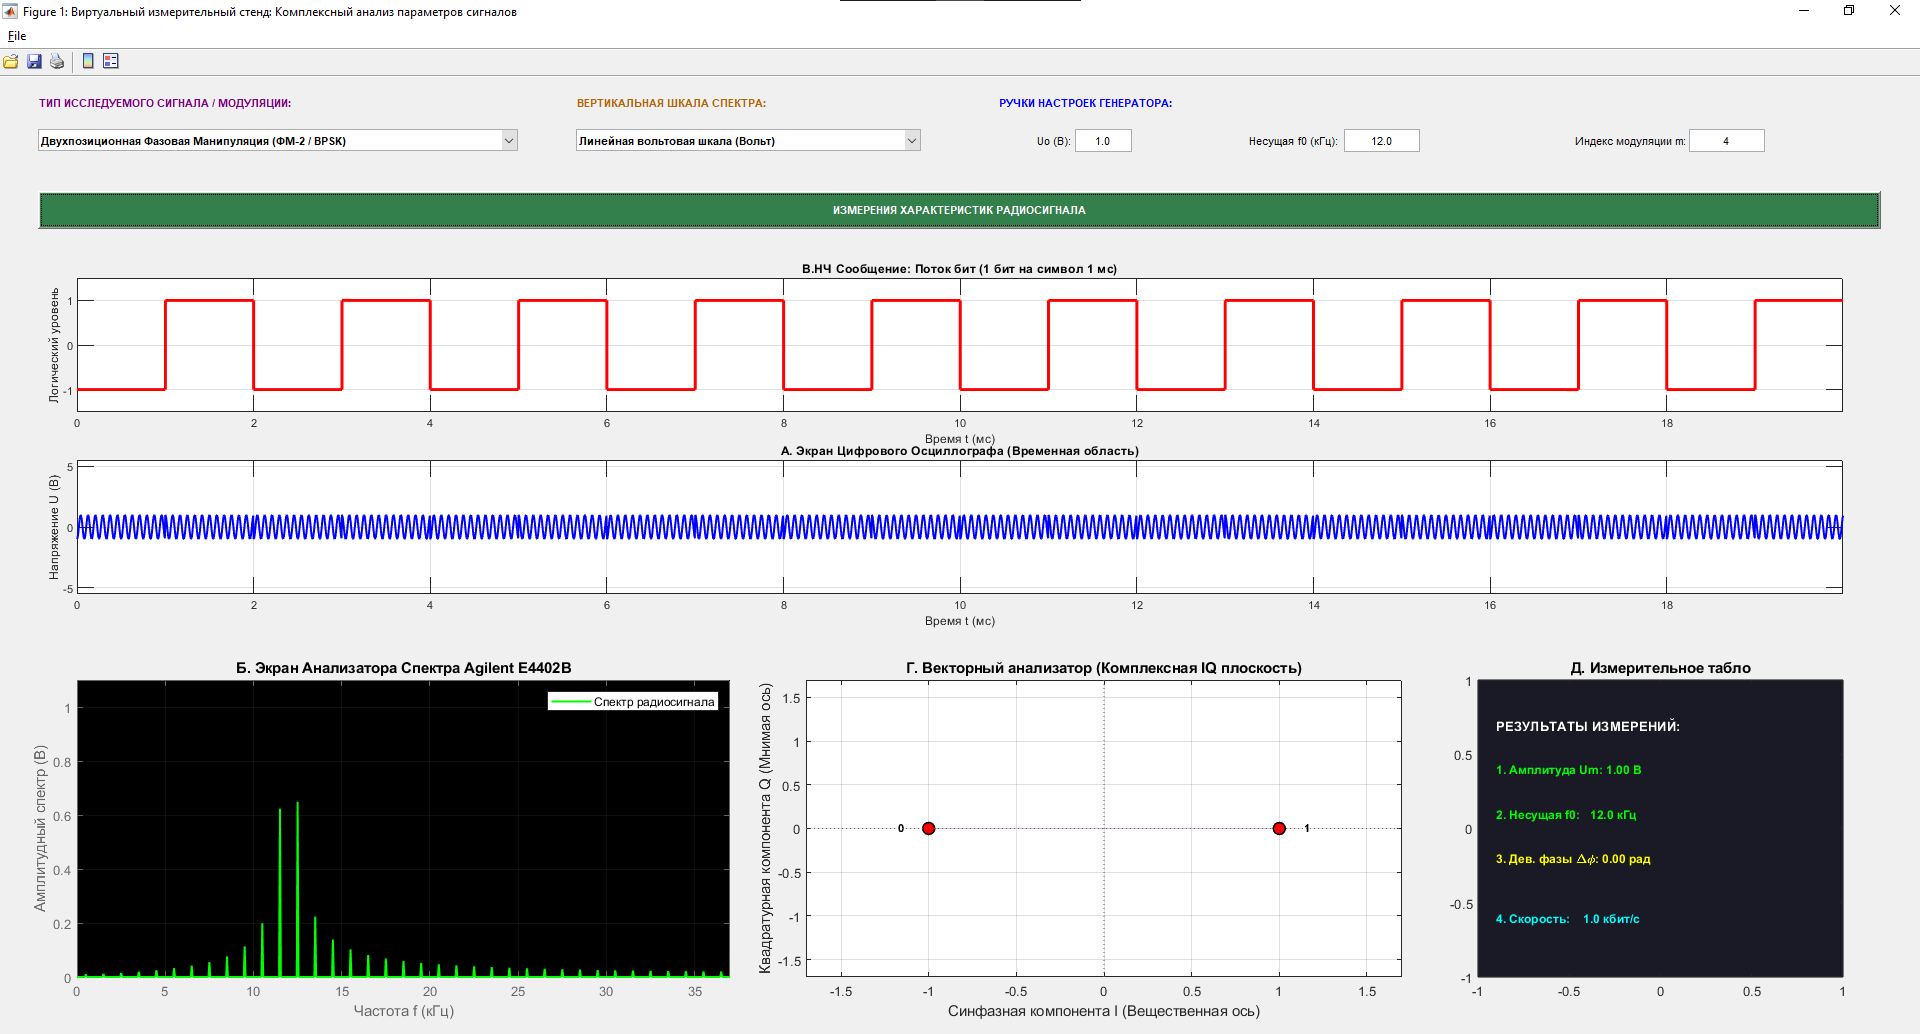
\includegraphics[width=1.0\textwidth]{images/BPSK}
    \caption{Результаты моделирования сигнала ФМ-2}
    \label{fig:BPSK}
\end{figure}

\section{Четырехпозиционная фазовая манипуляция}

\begin{figure}[H]
    \centering
    % Замените на имя вашего файла с графиком
    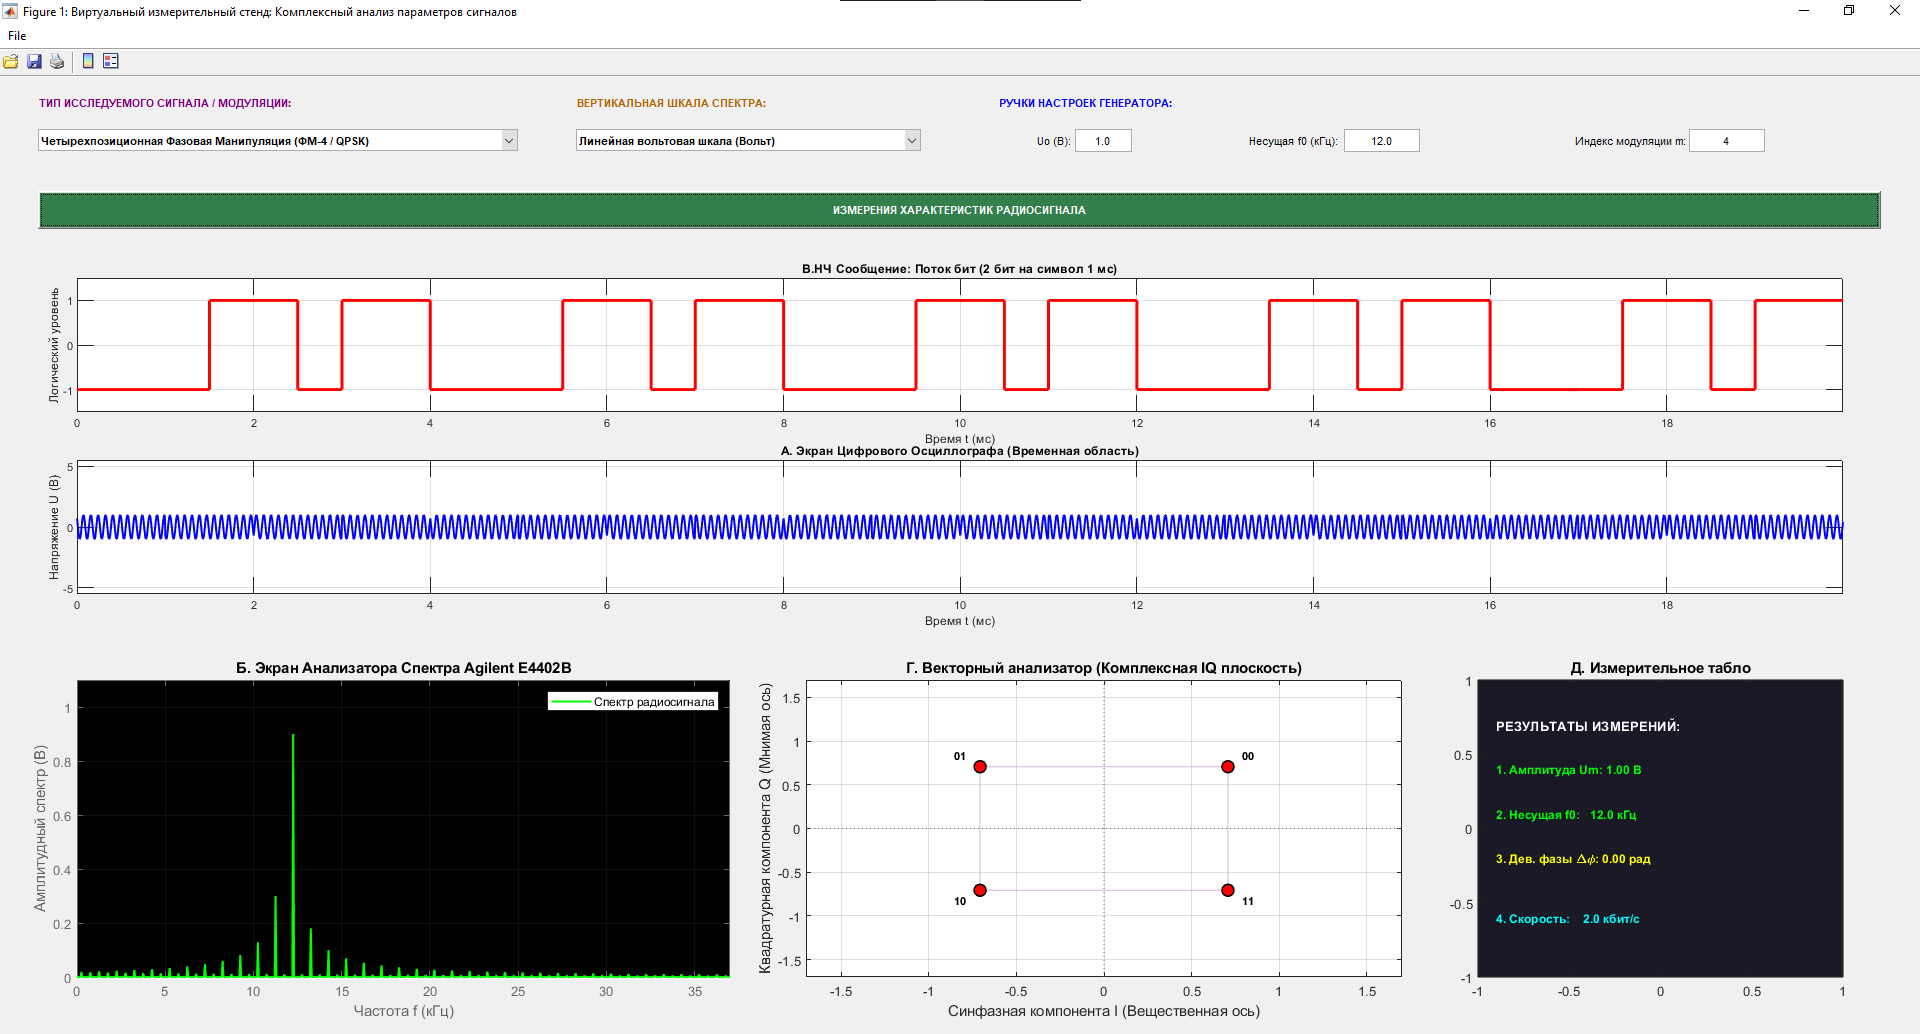
\includegraphics[width=1.0\textwidth]{images/QPSK}
    \caption{Результаты моделирования сигнала ФМ-4}
    \label{fig:QPSK}
\end{figure}

\section{Двухпозиционная частотная манипуляция}

\begin{figure}[H]
    \centering
    % Замените на имя вашего файла с графиком
    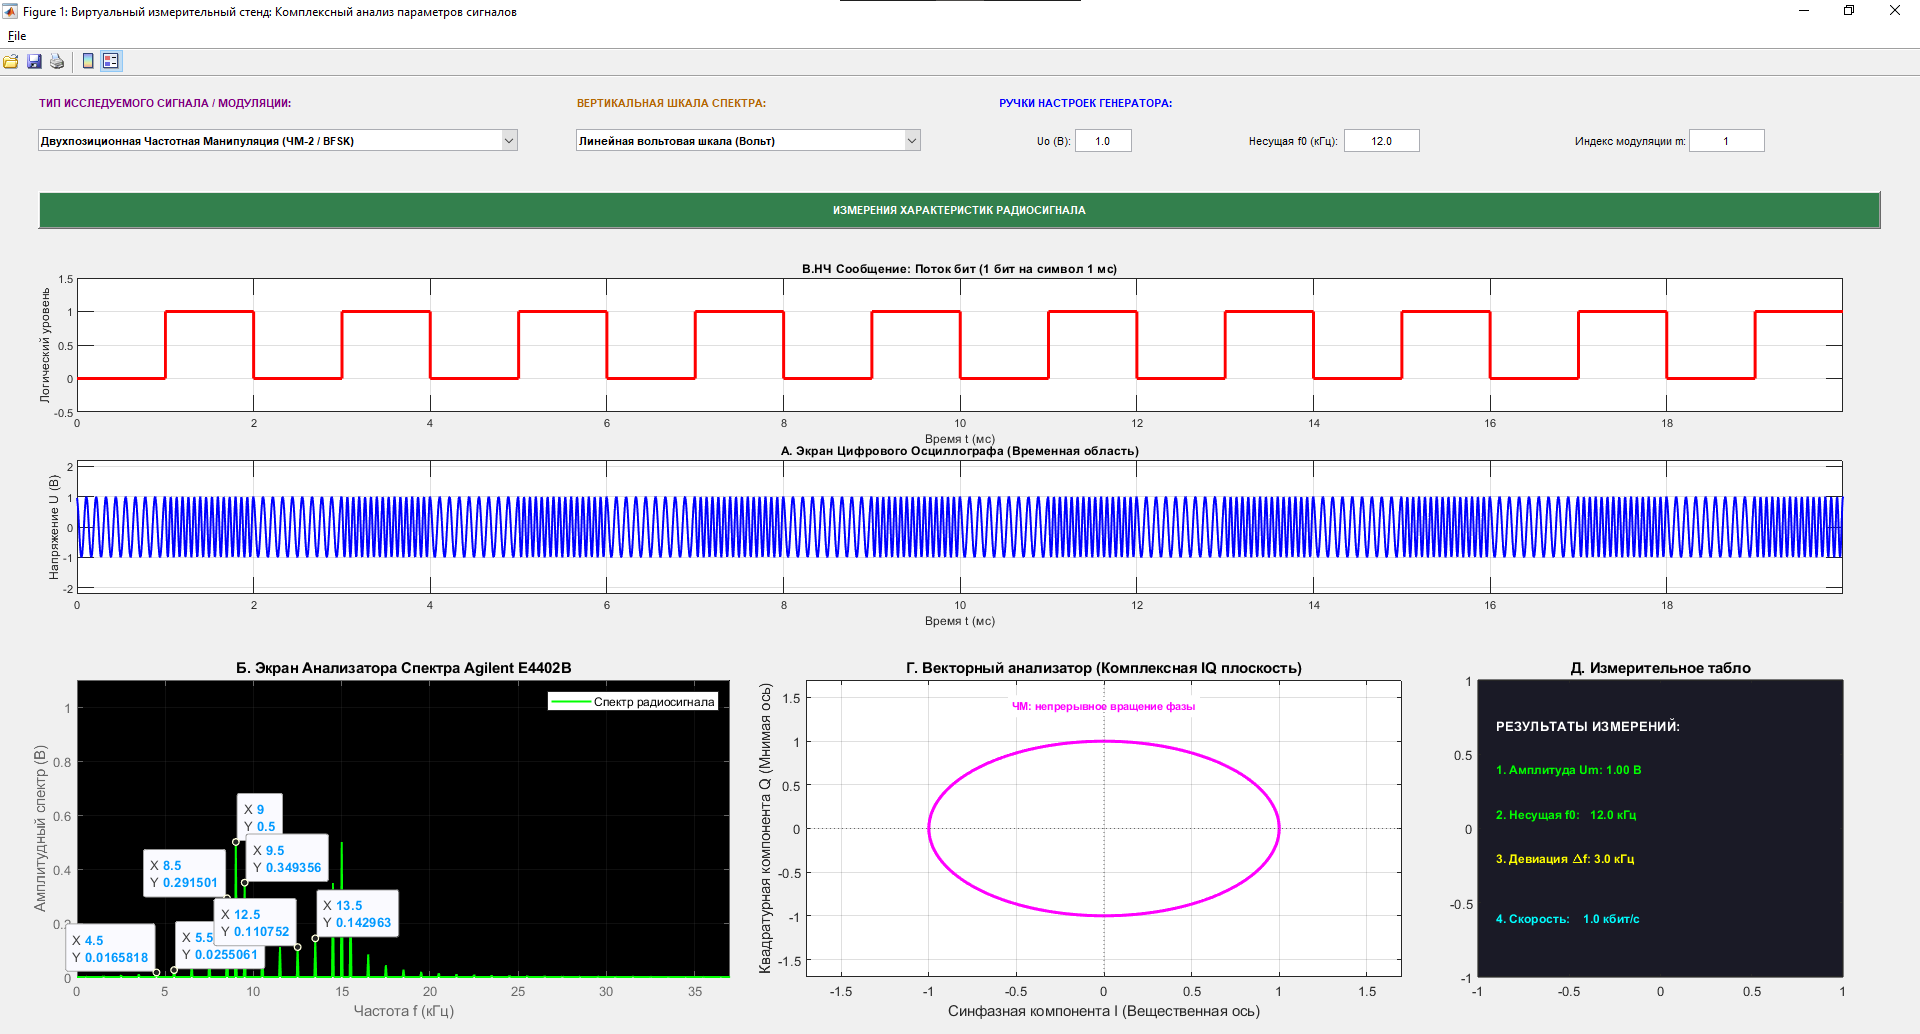
\includegraphics[width=1.0\textwidth]{images/FBSK}
    \caption{Результаты моделирования сигнала ЧМ-2 при $m = 1$}
    \label{fig:FBSK}
\end{figure}

\section{Четырехпозиционная частотная манипуляция}

\begin{figure}[H]
    \centering
    % Замените на имя вашего файла с графиком
    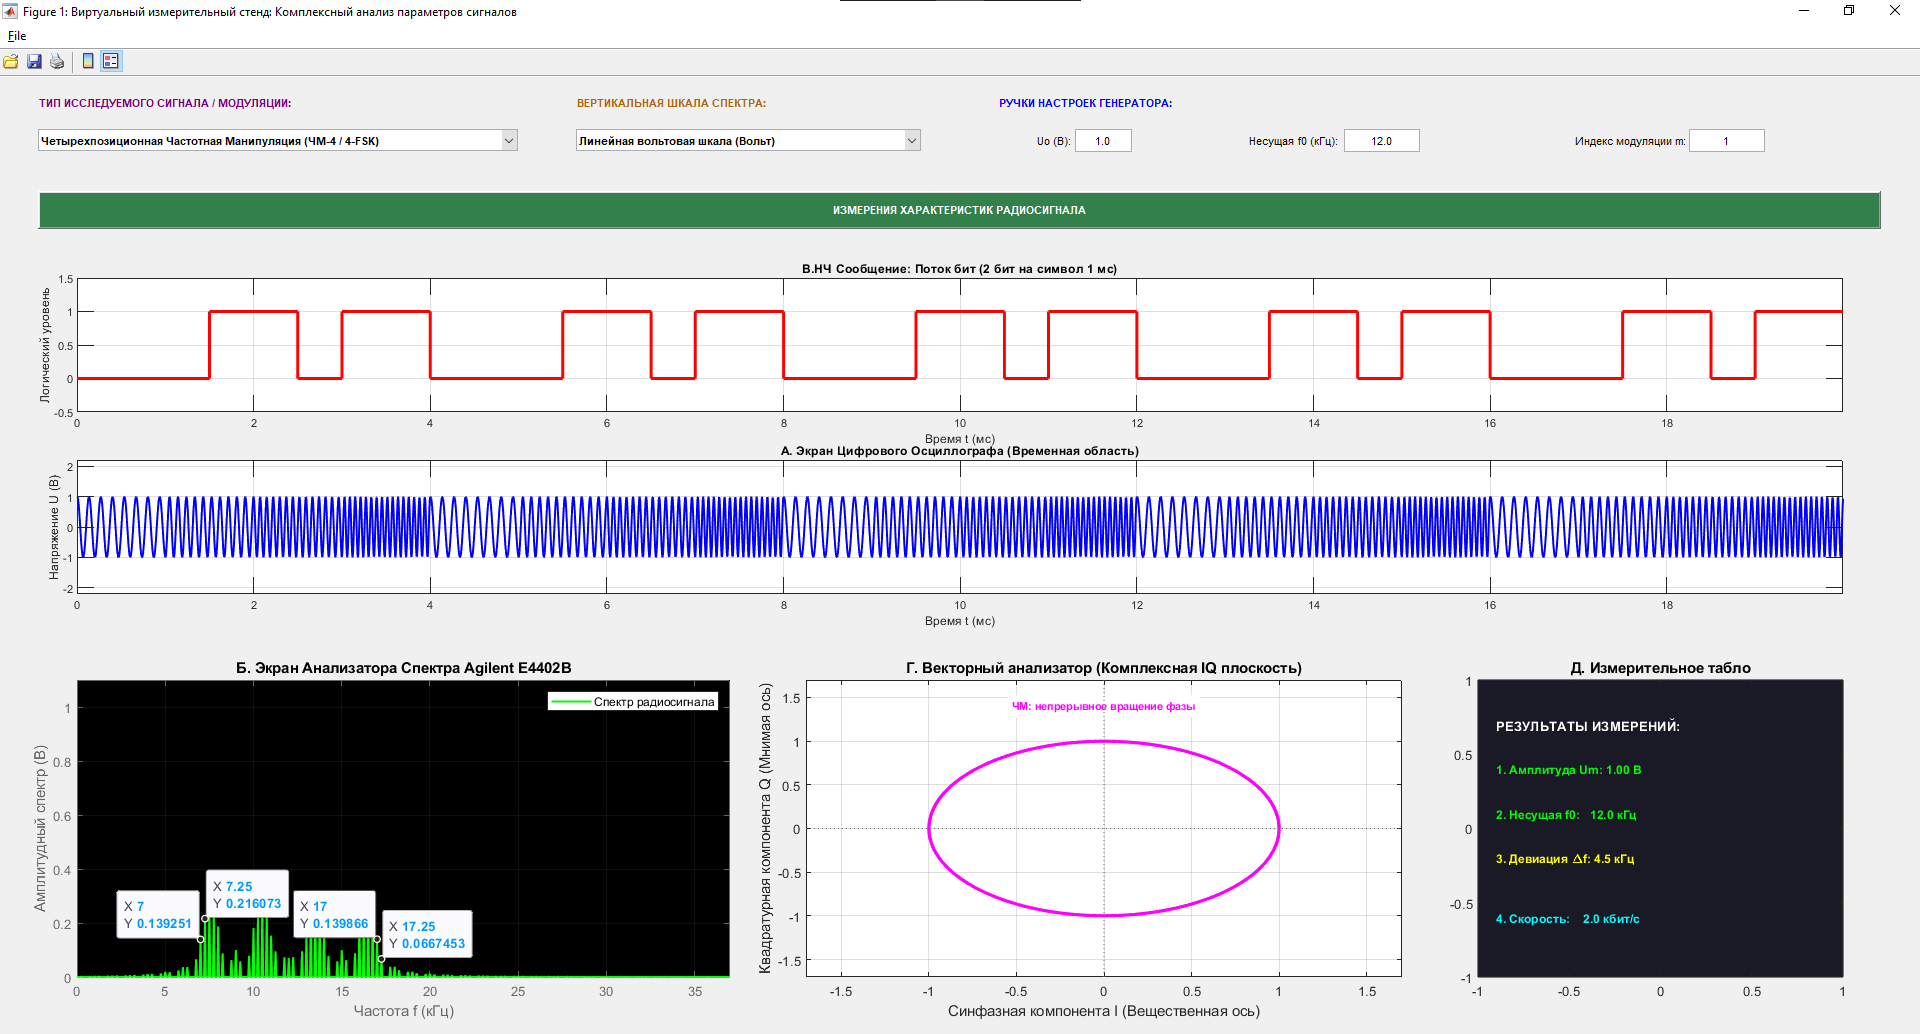
\includegraphics[width=1.0\textwidth]{images/FPSK}
    \caption{Результаты моделирования сигнала ЧМ-4 при $m = 1$}
    \label{fig:FPSK}
\end{figure}

\section{Амплитудно-фазовая манипуляция (АФМ-16)}

\begin{figure}[H]
    \centering
    % Замените на имя вашего файла с графиком
    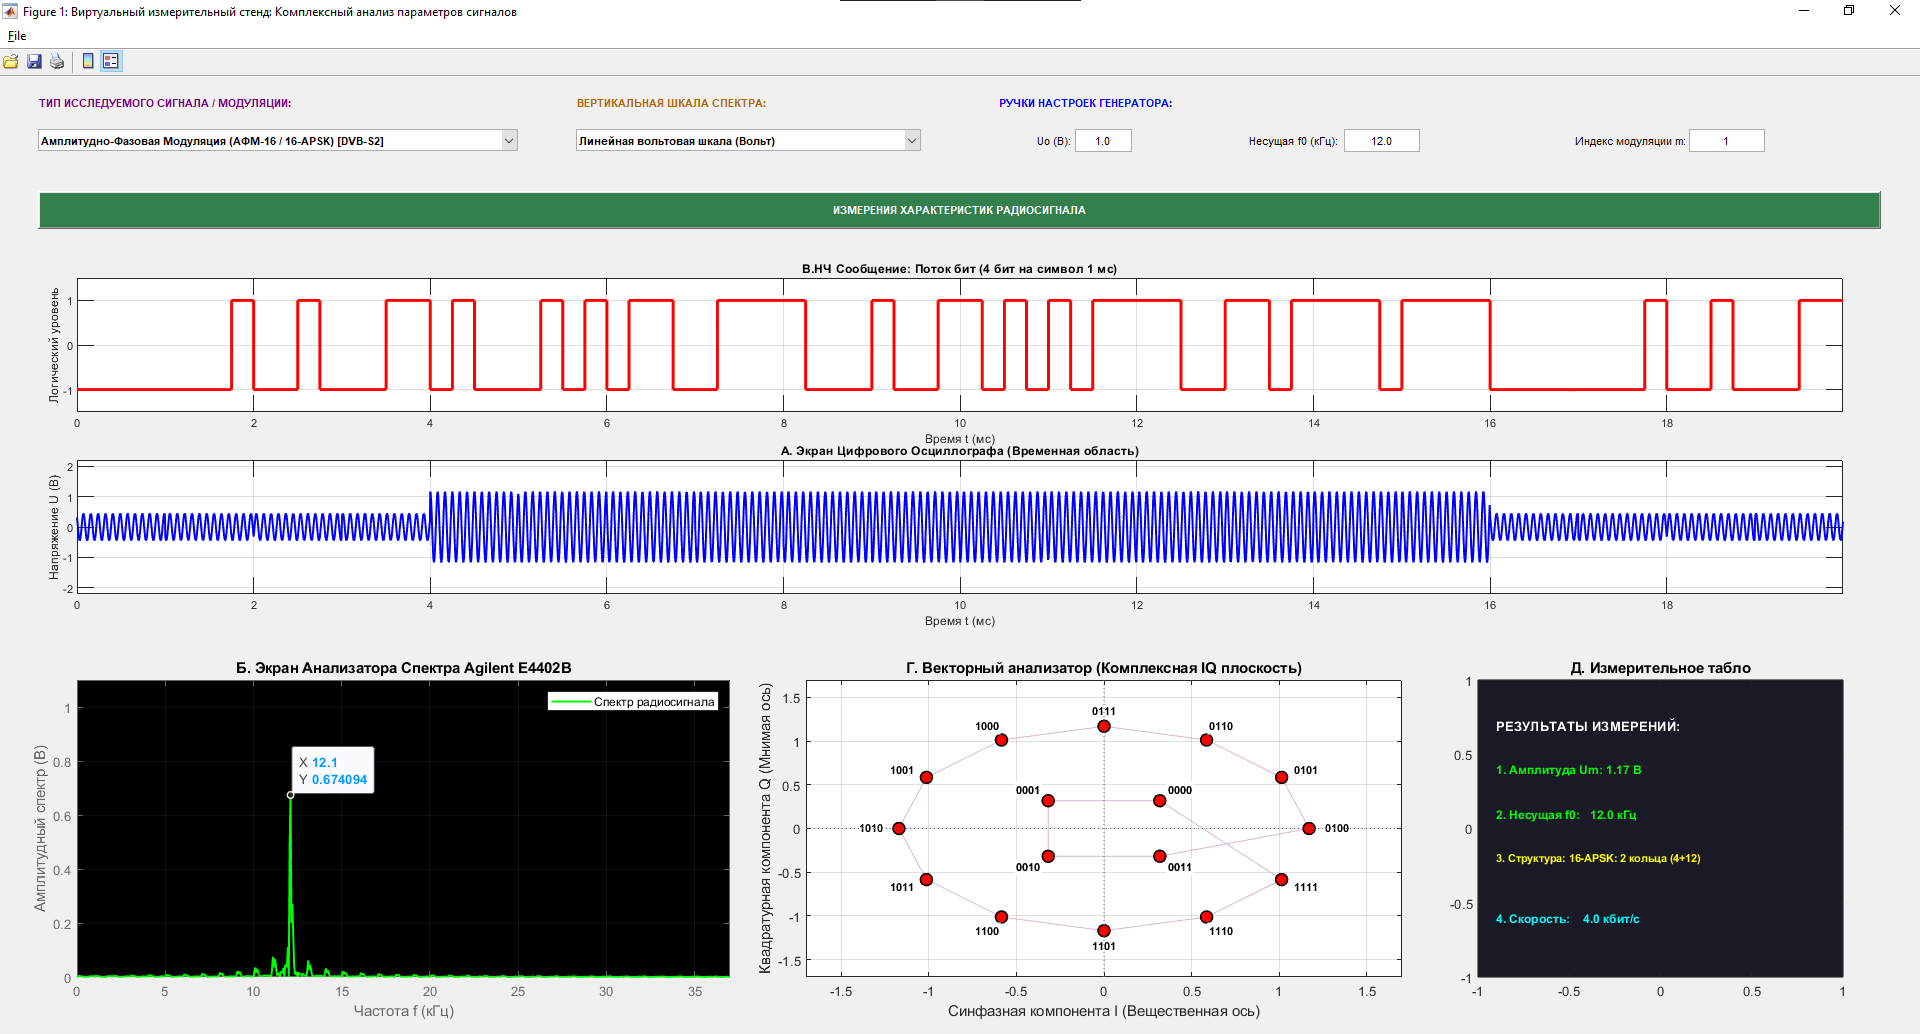
\includegraphics[width=1.0\textwidth]{images/APSK-16}
    \caption{Результаты моделирования сигнала АФМ-16}
    \label{fig:APSK-16}
\end{figure}

\section{Амплитудно-фазовая манипуляция (АФМ-32)}

\begin{figure}[H]
    \centering
    % Замените на имя вашего файла с графиком
    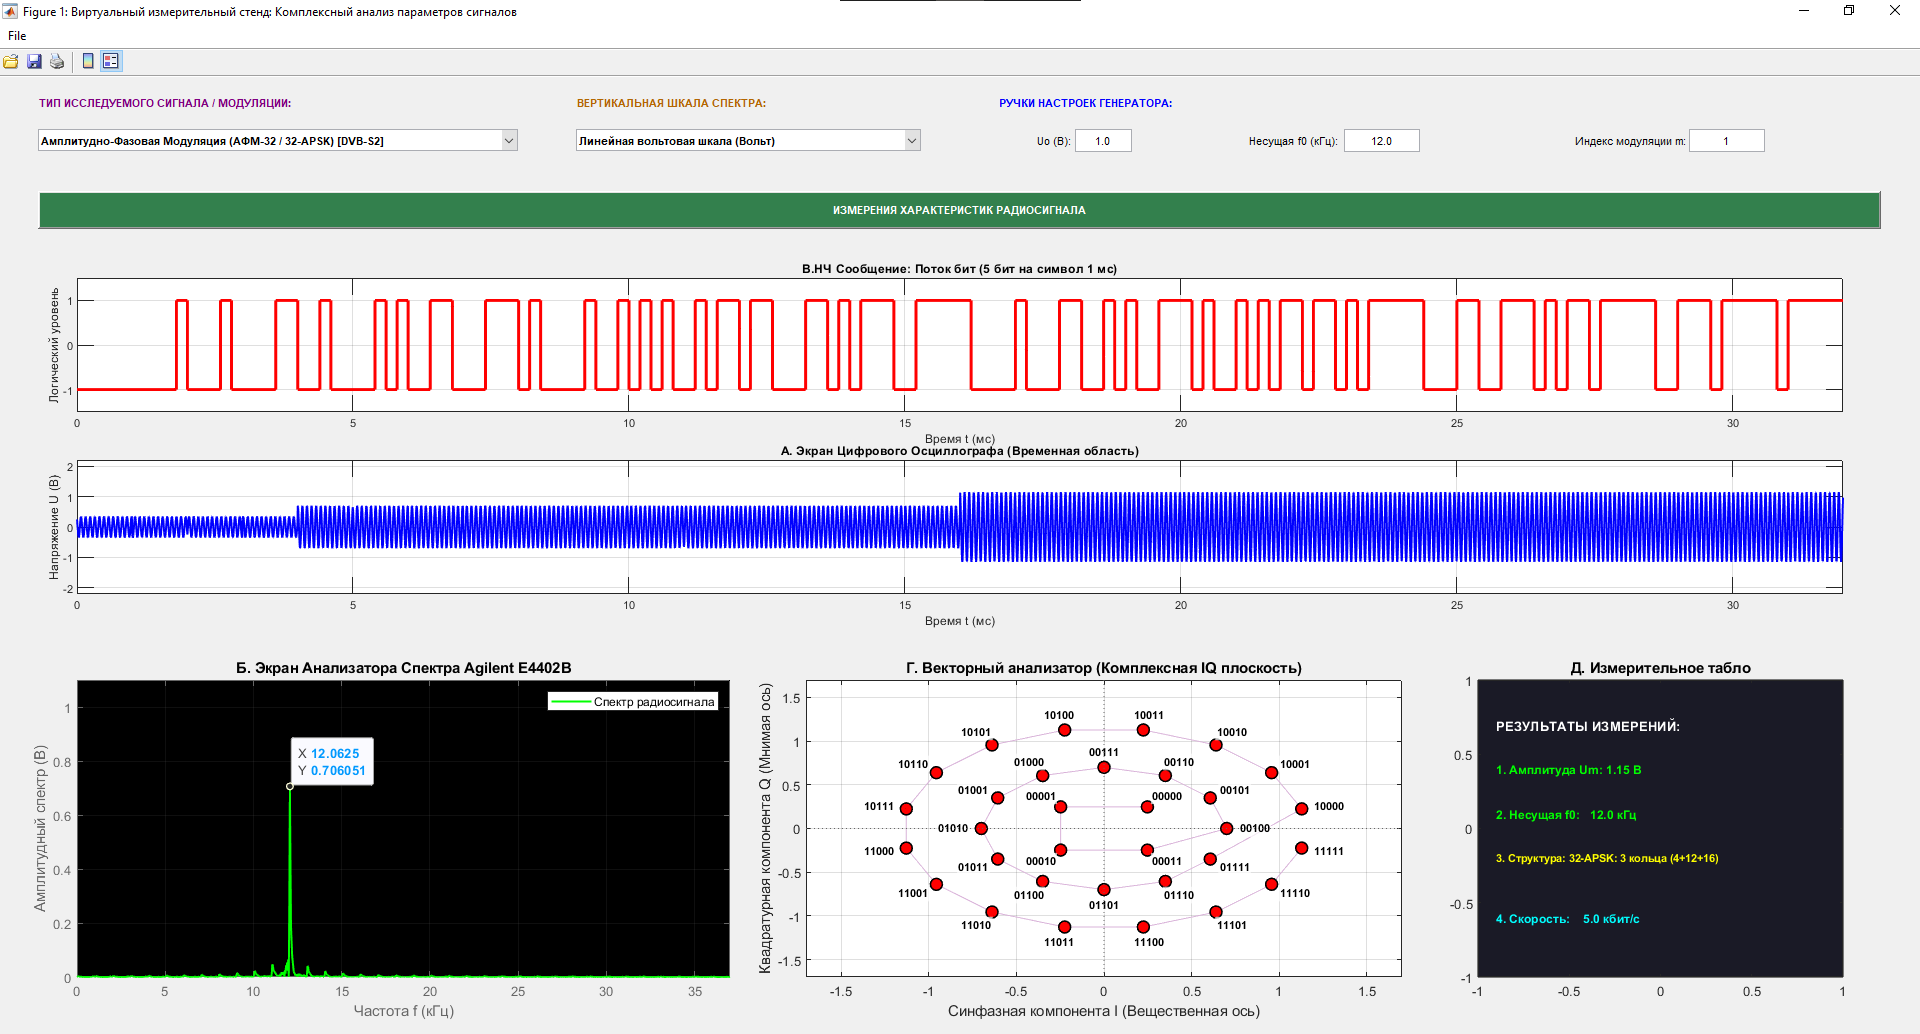
\includegraphics[width=1.0\textwidth]{images/APSK-32}
    \caption{Результаты моделирования сигнала АФМ-32}
    \label{fig:APSK-32}
\end{figure}

\section{Квадратурная амплитудная манипуляция (КАМ-16)}

\begin{figure}[H]
    \centering
    % Замените на имя вашего файла с графиком
    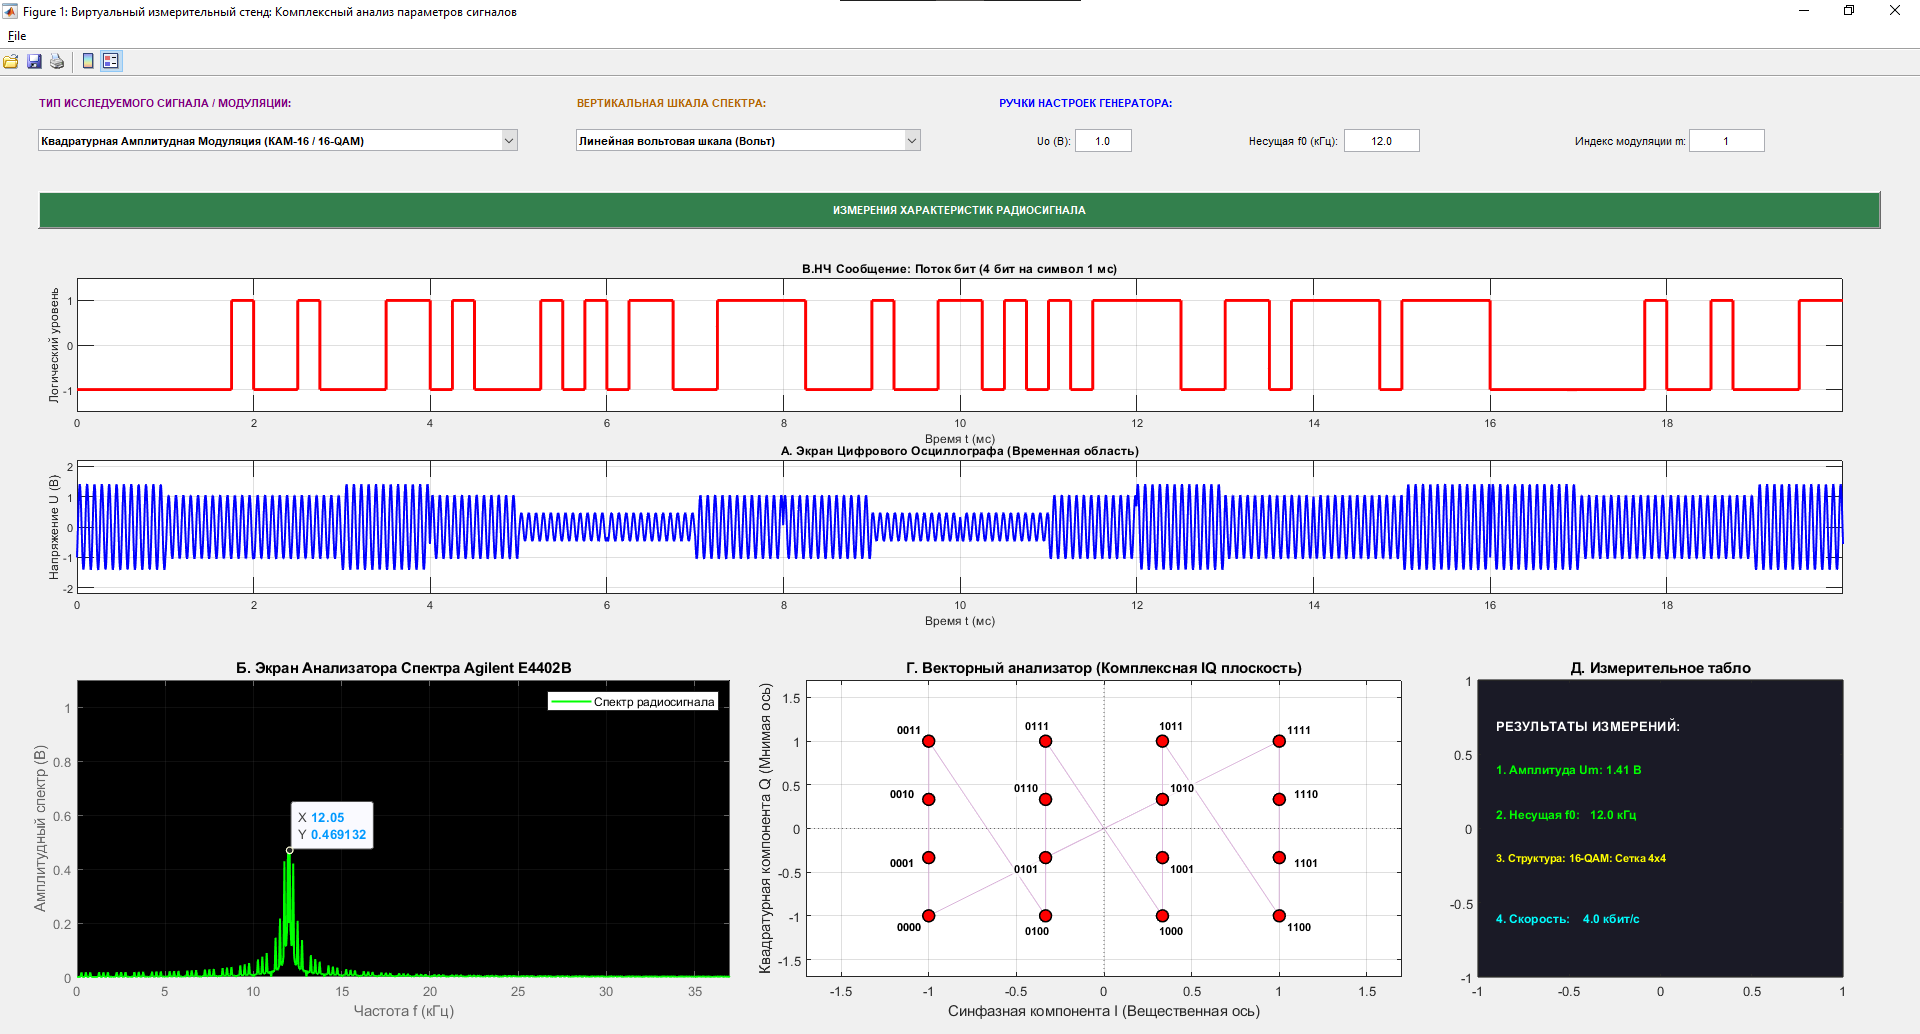
\includegraphics[width=1.0\textwidth]{images/QAM-16}
    \caption{Результаты моделирования сигнала КАМ-16}
    \label{fig:QAM-16}
\end{figure}

\section{Квадратурная амплитудная манипуляция (КАМ-32)}

\begin{figure}[H]
    \centering
    % Замените на имя вашего файла с графиком
    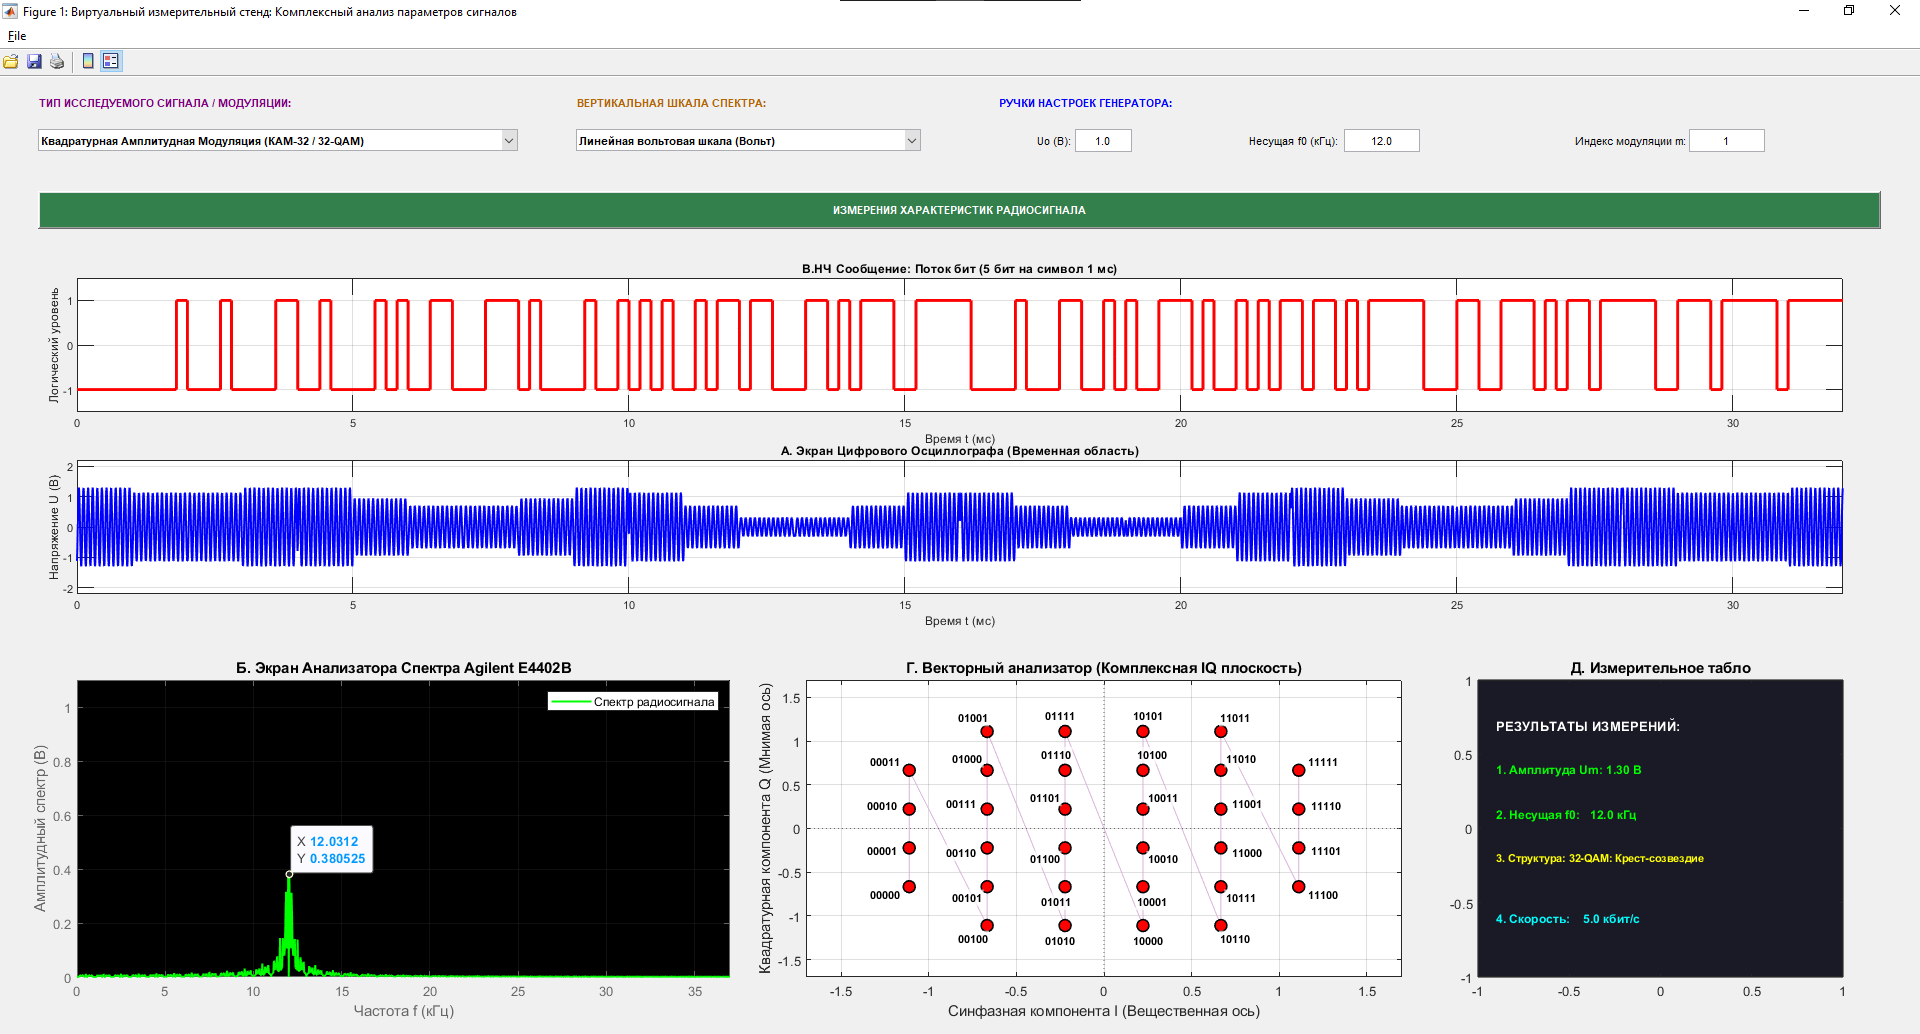
\includegraphics[width=1.0\textwidth]{images/QAM-32}
    \caption{Результаты моделирования сигнала КАМ-32}
    \label{fig:QAM-32}
\end{figure}